\problemname{Longest increasing pub-sequence}
\noindent

Elise har just börjat på Stackköpings Tekniska Högskola (STH), och som en del av mottagningen ordnas en traditionell pubrunda.
En pubrunda går ut på att man besöker alla sektionslokaler och dricker något på varje ställe.
Elise och hennes kompisar dricker inte alkohol, men däremot gillar de att gå långa sträckor.
Därför tänker de utforma en runda med så många besök som möjligt, sådan att avstånden de går mellan lokalerna är strikt ökande.
Din uppgift är att hitta maximala antalet besök de kan uppnå.

Sektionslokalerna finns på punkter i planet med heltalskoordinater.
Elise och hennes kompisar går alltid kortaste avståndet mellan två lokaler.
Avståndet är det vanliga Euklidiska, dvs. $\sqrt{(x_1 - x_2)^2 + (y_1 - y_2)^2}$.
De får börja vid vilken lokal som helst.
Det är tillåtet att besöka samma sektionslokal flera gånger, och det räknas som separata besök.
Däremot får de inte besöka samma ställe två gånger på raken.

\begin{figure}[!h]
\begin{center}
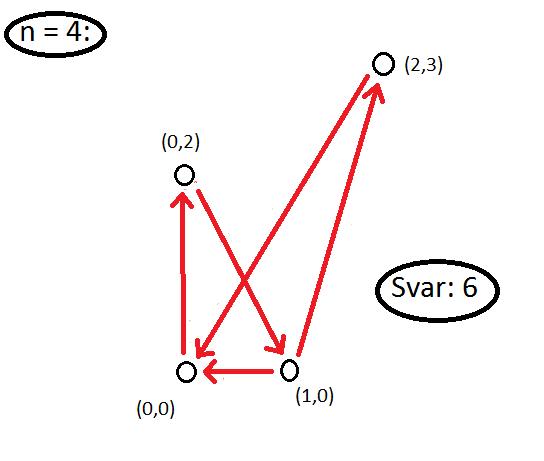
\includegraphics[width=8cm]{pubsequence.png}
\end{center}
\caption{Bilden föreställer Exempel 1. Om du startar vid $(1,0)$ och går längs med de röda pilarna får du en runda med $6$ besök, vilket också är det maximala antalet.}
\end{figure}

\section*{Indata}
Första raden innehåller ett heltal $N$ ($2 \leq N \leq 2000$), antalet sektionslokaler.
De följande $N$ raderna innehåller två heltal $x_i, y_i$ ($0 \leq x_i, y_i \leq 10^9$), koordinater för varje sektionslokal.

\section*{Utdata}
Skriv ut ett heltal, maximala antalet besök Elise och hennes kompisar kan göra om avstånden mellan punkterna är strikt ökande.

\section*{Poängsättning}
Din lösning kommer att testas på en mängd testfallsgrupper.
För att få poäng för en grupp så måste du klara alla testfall i gruppen.

\noindent
\begin{tabular}{| l | l | l |}
\hline
Grupp & Poängvärde & Gränser \\ \hline
$1$    & $10$         & $N \leq 3$ \\ \hline
$2$    & $10$         & $N \leq 5$ \\ \hline
$3$    & $30$         & $N \leq 200$ \\ \hline
$4$    & $50$         & Inga ytterligare begränsningar \\ \hline
\end{tabular}
